% This is "sig-alternate.tex" V2.0 May 2012
% This file should be compiled with V2.5 of "sig-alternate.cls" May 2012
%
% This example file demonstrates the use of the 'sig-alternate.cls'
% V2.5 LaTeX2e document class file. It is for those submitting
% articles to ACM Conference Proceedings WHO DO NOT WISH TO
% STRICTLY ADHERE TO THE SIGS (PUBS-BOARD-ENDORSED) STYLE.
% The 'sig-alternate.cls' file will produce a similar-looking,
% albeit, 'tighter' paper resulting in, invariably, fewer pages.
%
% ----------------------------------------------------------------------------------------------------------------
% This .tex file (and associated .cls V2.5) produces:
%       1) The Permission Statement
%       2) The Conference (location) Info information
%       3) The Copyright Line with ACM data
%       4) NO page numbers
%
% as against the acm_proc_article-sp.cls file which
% DOES NOT produce 1) thru' 3) above.
%
% Using 'sig-alternate.cls' you have control, however, from within
% the source .tex file, over both the CopyrightYear
% (defaulted to 200X) and the ACM Copyright Data
% (defaulted to X-XXXXX-XX-X/XX/XX).
% e.g.
% \CopyrightYear{2007} will cause 2007 to appear in the copyright line.
% \crdata{0-12345-67-8/90/12} will cause 0-12345-67-8/90/12 to appear in the copyright line.
%
% ---------------------------------------------------------------------------------------------------------------
% This .tex source is an example which *does* use
% the .bib file (from which the .bbl file % is produced).
% REMEMBER HOWEVER: After having produced the .bbl file,
% and prior to final submission, you *NEED* to 'insert'
% your .bbl file into your source .tex file so as to provide
% ONE 'self-contained' source file.
%
% ================= IF YOU HAVE QUESTIONS =======================
% Questions regarding the SIGS styles, SIGS policies and
% procedures, Conferences etc. should be sent to
% Adrienne Griscti (griscti@acm.org)
%
% Technical questions _only_ to
% Gerald Murray (murray@hq.acm.org)
% ===============================================================
%
% For tracking purposes - this is V2.0 - May 2012

\documentclass{sig-alternate}
\usepackage{fixltx2e,algpseudocode,pifont,graphicx}
\usepackage[linesnumbered,ruled,vlined]{algorithm2e}
\algrenewcommand\Return{\State \algorithmicreturn{} }%

\begin{document}
%
% --- Author Metadata here ---
\conferenceinfo{WOODSTOCK}{'97 El Paso, Texas USA}
%\CopyrightYear{2007} % Allows default copyright year (20XX) to be over-ridden - IF NEED BE.
%\crdata{0-12345-67-8/90/01}  % Allows default copyright data (0-89791-88-6/97/05) to be over-ridden - IF NEED BE.
% --- End of Author Metadata ---

\title{Spatial Alarms In Obstructed Space\titlenote{(Produces the permission block, and
copyright information). For use with
SIG-ALTERNATE.CLS. Supported by ACM.}}
%\subtitle{[Extended Abstract]
%\titlenote{A full version of this paper is available as
%\textit{Author's Guide to Preparing ACM SIG Proceedings Using
%\LaTeX$2_\epsilon$\ and BibTeX} at
%\texttt{www.acm.org/eaddress.htm}}}
%
% You need the command \numberofauthors to handle the 'placement
% and alignment' of the authors beneath the title.
%
% For aesthetic reasons, we recommend 'three authors at a time'
% i.e. three 'name/affiliation blocks' be placed beneath the title.
%
% NOTE: You are NOT restricted in how many 'rows' of
% "name/affiliations" may appear. We just ask that you restrict
% the number of 'columns' to three.
%
% Because of the available 'opening page real-estate'
% we ask you to refrain from putting more than six authors
% (two rows with three columns) beneath the article title.
% More than six makes the first-page appear very cluttered indeed.
%
% Use the \alignauthor commands to handle the names
% and affiliations for an 'aesthetic maximum' of six authors.
% Add names, affiliations, addresses for
% the seventh etc. author(s) as the argument for the
% \additionalauthors command.
% These 'additional authors' will be output/set for you
% without further effort on your part as the last section in
% the body of your article BEFORE References or any Appendices.

\numberofauthors{3} %  in this sample file, there are a *total*
% of EIGHT authors. SIX appear on the 'first-page' (for formatting
% reasons) and the remaining two appear in the \additionalauthors section.
%
\author{
% You can go ahead and credit any number of authors here,
% e.g. one 'row of three' or two rows (consisting of one row of three
% and a second row of one, two or three).
%
% The command \alignauthor (no curly braces needed) should
% precede each author name, affiliation/snail-mail address and
% e-mail address. Additionally, tag each line of
% affiliation/address with \affaddr, and tag the
% e-mail address with \email.
%
% 1st. author
\alignauthor
Dr. Tanzima Hashem\\
       \affaddr{Department of Computer Science}\\
       \affaddr{Bangladesh University of Engineering and Technology}\\
       \affaddr{Dhaka,Bangladesh}\\
       \email{tanzimahashem@gmail.com}
% 2nd. author
\alignauthor
Md. Touhiduzzaman \\
       \affaddr{Department of Computer Science}\\
       \affaddr{Bangladesh University of Engineering and Technology}\\
       \affaddr{Dhaka,Bangladesh}\\
       \email{tz08128@gmail.com}
% 3rd. author
\alignauthor
Sezana Fahmida \\
       \affaddr{Department of Computer Science}\\
       \affaddr{Bangladesh University of Engineering and Technology}\\
       \affaddr{Dhaka,Bangladesh}\\
       \email{sezanafahmida@gmail.com}
%\and  % use '\and' if you need 'another row' of author names
% 4th. author
%\alignauthor Lawrence P. Leipuner\\
 %      \affaddr{Brookhaven Laboratories}\\
  %     \affaddr{Brookhaven National Lab}\\
   %    \affaddr{P.O. Box 5000}\\
    %   \email{lleipuner@researchlabs.org}
% 5th. author
%\alignauthor Sean Fogarty\\
 %      \affaddr{NASA Ames Research Center}\\
  %     \affaddr{Moffett Field}\\
   %    \affaddr{California 94035}\\
    %   \email{fogartys@amesres.org}
% 6th. author
%\alignauthor Charles Palmer\\
 %      \affaddr{Palmer Research Laboratories}\\
  %     \affaddr{8600 Datapoint Drive}\\
   %    \affaddr{San Antonio, Texas 78229}\\
    %   \email{cpalmer@prl.com}
}
% There's nothing stopping you putting the seventh, eighth, etc.
% author on the opening page (as the 'third row') but we ask,
% for aesthetic reasons that you place these 'additional authors'
% in the \additional authors block, viz.
%\additionalauthors{Additional authors: John Smith (The Th{\o}rv{\"a}ld Group,
%email: {\texttt{jsmith@affiliation.org}}) and Julius P.~Kumquat
%(The Kumquat Consortium, email: {\texttt{jpkumquat@consortium.net}}).}
%\date{30 July 1999}
% Just remember to make sure that the TOTAL number of authors
% is the number that will appear on the first page PLUS the
% number that will appear in the \additionalauthors section.

\maketitle
\begin{abstract}

\end{abstract}

% A category with the (minimum) three required fields
\category{H.4}{Information Systems Applications}{Miscellaneous}
%A category including the fourth, optional field follows...
\category{D.2.8}{Software Engineering}{Metrics}[complexity measures, performance measures]

\terms{Theory}

\keywords{Spatial Alarm, Obstructed Space}
%\theoremstyle{plain}
\newtheorem{thm}{Theorem}[section] % reset theorem numbering for each chapter

%\theoremstyle{definition}
\newtheorem{defn}[thm]{Definition} % definition numbers are dependent on theorem numbers
\newtheorem{exmp}[thm]{Example} % same for example numbers

\section{Introduction}
The high availability of smart phones has led to the proliferation of location based services. According to many, the next step in location based services is Spatial Alarms. Many believe this particular feature is going to dominate the future mobile-phone computing systems. Spatial alarms are an extension of time-based alarms. It is, however, triggered by a specific location irrespective of time."Remind me if I'm within 100 meters of a pharmacy" is a possible example of a spatial alarm. It is a personalized location based service which can vary from user to user. Existing research has categorized spatial alarms into three types: public, shared and private. Public alarms are alarms which are active for every user within the system, such as an alarm must be sent to everyone within 100 meters of a building on fire. Private alarms are user defined alarms which can be viewed by the user, such as a user might set an alarm to alert her if she is within 100 meters of her favorite coffee shop. Shared alarms are shared between specific groups of people. In the previous example if a user chooses to share the alarm for the coffee shop with some of her friends it becomes a shared spatial alarm.\\
It is noteworthy that spatial alarms are quite dissimilar to spatial range query. Spatial alarms are based on a fixed location thus applying the techniques that are used in answering spatial range queries is both inefficient and wasteful for the two dominating reasons, Firstly, in spatial range query as the user is the main point of interest, continuous re-evaluation of her location is needed in case of a mobile user. In contrast, spatial alarms need only be re-evaluated when the user in approaching a specific location. Secondly, in spatial alarm, the main point of interest is a static location. So the user's location is not relevant at all times. It is quite clear that applying spatial range query techniques in evaluating spatial alarms is going to result in wastage of resources. If we start to evaluate spatial alarms as soon as the user is on the move even if the user is far away from her desired location our efforts will be futile. \\
Existing work in this area has focused mainly on Euclidean distance and road network models, to the best of our knowledge; no work is yet done on spatial alarms in obstructed space. Spatial alarm evaluation in obstructed space is different than road network or Euclidean space as it considers the obstacles in the path to the location of alarm. It is better approximated by a pedestrian scenario while road networks are approximated by vehicle scenarios. A vehicle can only go to a specific location following a predefined road, but a pedestrian's path is not limited by roads. However, a pedestrian is obstructed by various obstacles such as buildings or trees. So while calculating the distance from spatial alarms, we have to consider the obstructed distance.\\
Spatial alarms are location-based, user-defined triggers which will possibly shape the future mobile application computations. They are distinct from spatial range query and do not need immediate evaluation after the user has activated them.The spatial alarm evaluation strategies are judged based on two features, High accuracy and High system scalability. High accuracy refers to the quality that guaranties no alarms are missed. And High scalability is the feature that ensures that the system can adapt to a large number of spatial alarms.
In this paper, We propose a novel approach to evaluate spatial alarms in obstructed space which ensures both high accuracy and high scalability.


\section{Problem Setup}
\textit{Obstructed Space Route Problem} denotes the problem of finding the shortest route between two query-points  in Obstructed Space where non-intersecting 2D polygons represent \textit{obstacles} and where the route does not traverse through any obstacles.The length of the Obstructed route between points a and b is called the \textit{Obstructed Distance} between a and b, denoted by D\textsubscript{obs,a,b}.\\
A \textbf{Spatial Alarm Query in Obstructed Space} is formally defined as follows:
\begin{defn}
Given the user's current location $q$,and an alarming distance $u_d$ for an alarm, spatial alarm query returns the set of alarms $P$, where for each $p \in P, D_{obs,q,p} < u_i$. 
\end{defn}
We define three different type of regions: \textit{Known Region}, \textit{Reliable Region} and \textit{Safe Region} to provide spatial-alarm in an obstructed space to the client accurately and efficiently.

\begin{defn} 
\textbf{Known Region:} We define two known regions for the POIs and the obstacles separately. The region containing at least 1 POI is the known region for POI.\\
The region circulating the POIs' known region containing none or single colliding obstacles is the known region for the obstacles.The set of obstacles and POIs within this region is known to the client. 
We will denote the radius of the known region of the POIs as $r_{kp}$ and that of the obstacles as $r_{ko}$.
\end{defn}

\begin{defn}
\textbf{Reliable Region:} Within which region, no further query to the server has to be done to compute a consistent set of answers, that is termed as a reliable region. Given the radius of the reliable region as $r_{rel}$, the user's previous location as $q$ and the current location as $q'$, if $\vert q-q'\vert < r_{rel}$, then by this definition no further queries to the server has to be done to compute a consistent set of answers.
\end{defn}

\begin{defn} \label{def:safe_region}
\textbf{Safe Region:} A safe region is the region located inside reliable region within which the answer set of POIs remains unchanged for a moving client. This region can also be called a hibernation-region, since the client just hibernates without doing any literal calculation while it's inside this region. We will denote the radius of the safe region as $r_{safe}$. Given the user's previous location $q$ and the current location $q'$, if $\vert q-q'\vert < r_{safe}$, then no calculation is needed to compute the answer set.
\end{defn}
 
The \textsc{GetAllPOI}($q, R_{max},P_{max}$) function populates the set P of POIs within maximum of $R_{max}$ radius centring the query point (client's current location) $q$ and with a maximum count of $P_{max}$. Similarly, \textsc{GetObstacleSet}($q, R_{max},O$) function returns the set of all obstacles within maximum of $R_{max}$ radius centring $q$, but except those in a previous obstacle set O given as the third parameter. \\
Instead of the very naive \textsc{GetAllPOI}($q, R_{max},P_{max}$), a modified function \textsc{CheckNewPOI}$(q, r_{k}, P)$ is used in our later approaches to retrieve all excluded POIs of the given set P within the radius $r_{k}$ centring the point $q$. \\
\textsc{MakeVisGraph}$(P,O)$ function returns the \textit{visibility graph} $V_G$ with the set of POIs $P$ and obstacles $O$.\\
Here, a \textbf{Visibility Graph} is a graph $V_G(V,E)$ where each $v \in V$ is either a POI or a data-point and for each $(u,v) \in E$, there is an edge $e$ between $u$ and $v$ if and only if it does not intersect with any obstacles $i.e.$ $u$ and $v$ are \textit{visible} to each other along the edge $e$. \\
\textsc{AlarmUser}$(p_i)$ triggers an alarm to the user since the alarm (POI) $p_i$ is reached and also marks $p_i$ to be reached in the set of POIs $P$. \\  
Moreover, \textsc{EuclideanDist($q, q'$)} returns the Euclidean distance between the two points $q$ and $q'$, whereas \textsc{ObsDist}($q, q', V_G$) returns the obstructed distance between the points $q$ and $q'$ computed from the visibility graph $V_G$.
\\ In the final approach, two more functions returning boolean value are used as \textsc{isAnyPoiUnreachable}($V_G$) and \textsc{isPathInside}($q, p_i, r_{safe}, V_G)$. The function \textsc{isAnyPoiUnreachable}($V_G$) returns true if any POI inside the visibility graph $V_G$ cannot be reached along any path inside $V_G$. Another function, \textsc{isPathInside}($q, p_i, r_{safe}, V_G)$ returns true if the POI $p_i$ is inside the radius $r_{safe}$ centring $q$ within the visibility graph $V_G$ along with all of its connecting edges from the center $q$, otherwise returns false.
\\ Notations used in describing the algorithms follow the fact that all Euclidean distance related variables are in small letters whereas the variables related to obstructed distance are in capital letters.
 
\section{Related Work}
Extensive research has been performed and various  effective algorithms have been proposed \cite{roadalarm},\cite{mur},\cite{bamba} to process spatial alarms in Euclidean space and road network in recent years. Euclidean space considers the straight line distance between two points irrespective of obstacles on the other hand in road networks navigation is limited along predefined roads.\\ Obstructed space considers the shortest distance between two points in the presence of obstacles. Various spatial range query algorithms have been presented in recent times \cite{obst1},\cite{obst2},\cite{ognn} such as nearest neighbor and group nearest neighbor in obstructed space.\\
Again, comprehensive research \cite{liu} has been conducted to make spatial alarm evaluation energy-efficient and effective in road networks. 
However, to the best of our knowledge no research work has yet been published on the topic of spatial alarms in obstructed space.
\\

% Our algos : 3 sections mainly - Naive, modified naive & the final approach
\section{Naive Approaches}
To compare the efficiency of our approach, we are about to represent two straightforward solutions for processing spatial-alarms in an obstructed space - sequential alarm (POI) processing in regular basis and region-divided alarm (POI) processing. 
Both of these algorithms are stated and explained in the following subsections.


\subsection{Sequential Processing on Regular Basis}
The POIs are saved in an R-tree indexed by own distance from the query point. In this naive approach, a maximum number of nearest POIs are retrieved from the server and on a minimum change of the user's location, a system event will fire an update procedure checking whether to give any alarm to the client or not along with the check of necessity to fetch more POI and obstacle when the client goes outside of the farthest POI's alarming zone.

%\begin{algorithm}
\DontPrintSemicolon

%\begin{algorithmic}[1]
\begin{algorithm}
\caption{\textsc{InitNaive1}($q$, $r_{max}$, $p_{max}$)}
    \SetKwInOut{Input}{Input}
    \SetKwInOut{Output}{Output}
    \Input{Query point $q$, Max search radius $r_{max}$, max no. of POIs $p_{max}$}
    \Output{Answer set $A$} 
	
	 $P \gets \textsc{GetAllPOI}(q, r_{max}, p_{max})$ \;
	 $O \gets \textsc{GetObstacleSet}(q, r_{max}, \emptyset)$ \;
	 $V_G \gets \textsc{MakeVisGraph}(P, O)$ \;
	 $u_{min} \gets \infty$\;
	
	\For{$i \gets 1$ to $\left\vert{P}\right\vert$}{
		 $u_{min} \gets min( u_{min}, u_i )$ \; 
	}
	$k_{min} \gets (r_{max} - u_{min})$ \\
	\Return $A \gets \textsc{MakeAnswerSet}(q, k_{min}, P, O, V_G)$ \;
\end{algorithm}

\begin{algorithm}
\caption{\textsc{UpdateNaive1}$(q', A)$}

    \SetKwInOut{Input}{Input}
    \SetKwInOut{Output}{Output}
    \Input{$q', A$}
    
     $q_d \gets \textsc{EuclideanDist}(q, q')$\;
	 \For{$i \gets 1$ to $\left\vert{P}\right\vert$}{
		\If{$\textsc{EuclideanDist}(q', p_i) > u_i$}{
			$\textsc{AlarmUser}(p_i)$\;
		}
	}
	 \If {$q_d > k_{min}$ }{
		call \textsc{InitNaive1}$(q', 100, 100)$
	}
\label{UpdateNaive1}
%\end{algorithmic}
\end{algorithm}


%The run-time of the first line of the second procedure \ref{UpdateNaive1} is $O(\left\vert{P}\right\vert)$, whereas the second line depends on the amount of location-change and the FetchPOI procedure.
In this approach, the visibility-graph construction requires $O(n^2)$ \cite{mur}, where $n =$ the number of edges of the obstacles and this algorithm is run more often from the update algorithm. A huge overhead is also sufficed to make P and O sets using such procedure. Again, The algorithm \ref{UpdateNaive1} can also be run much less time than in this approach, which is improvised in the later approaches.
\\Moreover, the accuracy of this naive approach is vulnerable to many cases which are explained and handled in the following approaches one by one.


\subsection{Region-based Alarm Processing}
This naive approach is a region-based modified straight forward approach which searches for a new alarm inside the known region as soon as the client changes it's position.
This naive algorithm works in three parts - the first one retrieves all POI and obstacles and then computes the known and reliable regions, the second one calculates the visibility graph and periodically checks the client status to give alarms for any POI after every hibernation-period expiration and the third procedure checks the region crossings to recompute the answer set on any minimal location-change of the client.
The algorithms \ref{InitRegionBase},\ref{SafeRegionCalc},\ref{OnLocationChange} show the respective parts.\\
The input to the algorithm \ref{InitRegionBase} is the current location of the user $q$ and the increment delta, the amount by which the regions will be expanded , $r_d$. The output of the algorithm is an answer set A which consists of the set of all obstacles $O$ and POIs $P$ along with the respective visibility graph $V_G$ within the known-region radius $r_{k}$ centring $q$.

\begin{algorithm}
\caption{\textsc{InitRegionBase}($q,r_d$)}
\label{InitRegionBase}
%\begin{algorithmic}[1]
%\Procedure{InitRegionBase}{}

    \SetKwInOut{Input}{Input}
    \SetKwInOut{Output}{Output}
    \Input{Query point $q$, increment delta $r_d$}
    \Output{The answer set, $A=\left\{ { r_k, P, O}\right\}$}
    
	\While {$\left\vert{P}\right\vert < 1$ }{
	    $r_k \gets (r_k + r_d) $\;
	    $P \gets \textsc{CheckNewPOI}(q, r_{k}, P) $
	}
	 $O \gets \textsc{GetObstacleSet}(q, r_k, \emptyset)$\;
	 $V_G \gets \textsc{MakeVisGraph}(P, O)$	\;
	 \Return $A = \textsc{MakeAnswerSet}(r_k, P, O, V_G)$ 
%\EndProcedure
\end{algorithm}

The input to the algorithm \ref{SafeRegionCalc} is the current location of the client $q$ and the answer set from the algorithm \ref{InitRegionBase}. This algorithm is also responsible for triggering an alarm to the client, if s/he is within the alarming distance of any POI.

\begin{algorithm}
\caption{\textsc{SafeRegionCalc}($q,A$)}
\label{SafeRegionCalc}
    \SetKwInOut{Input}{Input}
    \SetKwInOut{Output}{Output}
    \Input{Query point $q$, answer set $A$}
    \Output{$r_{safe}$}
    
	 \If {$\textsc{isAnyPoiUnreachable}(V_G)$}{
		$A \gets $ \textsc{InitRegionBase}($q, 10$) \;
		call \textsc{SafeRegionCalc}($q, A$)
	}
	
	 $u_{min} \gets \infty, u_{max} \gets 0$ \\
	 \For{$i \gets 1 to \left\vert{P}\right\vert$}{
	 	$D_i \gets \textsc{ObsDist}(q, p_i, V_G) $ \;
		$D_{min} \gets min( D_{min}, D_i )$ \;
		$D_{max} \gets max( D_{max}, D_i )$ \;
	}
	 $r_{rel} \gets ( r_k - D_{min} )$\\
	 \ForEach{$p_i \in P$}{
		\If {$\textsc{ObsDist}(q, p_i, V_G) < u_{i}$} {
			\textsc{AlarmUser}($p_i$)
		}
	}
	 \Return $r_{safe} \gets (D_{min}-u_{max})$ 
%\EndProcedure
\end{algorithm}

The input to the algorithm \ref{OnLocationChange} is the current and the previous location of the client ($q'$ and $q$), the radius of the safe region($r_{safe}$), the reliable region($r_{rel}$) and the known region($r_{k}$) and finally the already computed answer set $A$. The output of the algorithm is the minimum distance $d_u$ to trigger this algorithm the next time.

\begin{algorithm}
\caption{OnLocationChange($q, q', r_{safe}, r_{rel}, r_k$)}
\label{OnLocationChange}
    \SetKwInOut{Input}{Input}
    \SetKwInOut{Output}{Output}
    \Input{$q, q', r_{safe}, r_{rel}, r_k, A$}
    \Output{$d_u$}
    
    $q_d \gets \textsc{EuclideanDist}(q, q')$
    
    \If{$q_d > r_{rel}$}{
    		$A \gets \textsc{InitRegionBase}(q, q_d)$ \;
    		call \textsc{SafeRegionCalc}($q, A$) \;
    }
    \ElseIf{$q_d > r_{safe}$}{
    		call \textsc{SafeRegionCalc}($q, A$) \;
    }
    
    \Return $d_u = r_{safe}$
%\EndProcedure
%\end{algorithmic}
\end{algorithm}

In this approach, more than one query for the known region computation has to be done frequently to the server after computing the visibility graph and if any unreachable POI is found out - which seems very much inefficient.
\\ Moreover, the safe region is in its minimum size in this approach, which requires more computation in the client side and so gets the approach less efficient.
\\ These problems are solved in the following final approach.

\section{Spatial Alarm in Obstructed Space}
Our spatial alarm evaluation system is divided into client-server architecture. The server has access to the locations of mobile users, location of alarms and location of obstacles. In this paper we assume that all users have access to some sort of localization service such as GPS or Wi-Fi that allow the server to pinpoint their current location. The client application is a thin-weight application that communicates with the server at regular intervals to retrieve necessary information about alarms and the obstacles. With the help of the client application the users can personalize their alarms as public, private or shared. They can join any public alarm or shared alarm as per their choice. We assume that the user can use any device such as smart-phones or PDA.\\ Our aim is to provide an energy-efficient, concise and accurate spatial alarm service for obstructed space. To preserve energy, the popular approach is to put the device in use to a low-power consumption state or sleep state. We propose a novel approach of computing a \textit{safe region}. As long as the client device is in the safe region, the device can be put into sleep state without the risk of any alarm being missed. \\

Spatial alarm evaluation can be optimized using two key features: firstly, reducing the number of device wake-ups and secondly reducing the re-computation of same obstructed distance and reducing the number of duplicate data retrieval from the server. For the first strategy to be successful our safe-region computation should be accurate and optimal. We propose an algorithm in the section which will compute an optimal safe-region for our spatial alarm evaluation system. The second optimization technique is related to the safe-region computation technique. To compute the safe region the client application must communicate with the server as it needs the location of obstacles and alarms. In this paper we aim to optimize this communication by ensuring that no redundant data is retrieved from the server. We propose two different type of strategies which highlight exactly one of the aforementioned key features. Our application has two different modes,namely, \textit{Bandwidth Saving Mode} and \textit{Computational Cost Saving Mode}

\subsection{Bandwidth Saving Mode}
In this mode the main focus is to reduce the bandwidth of communication between the server and the client. This mode is designed to operate in three parts - \textit{client-initialization}, \textit{alarm-configuration} and \textit{update on any location change}. Algorithm \ref{ClientInit}, \ref{ConfigAlarm}, \ref{ULC} show the algorithmic-steps for these three parts respectively.

The input to the client-initialization algorithm (algorithm \ref{ClientInit}) is the current location of the client $q$ and the incremental radius $r_d$ by which the radius of the searchable region will expand. This algorithm improvises the single known region concept of the second naive approach described above into two different known regions for POIs and obstacles, which makes the frequent queries more efficient and accurate and needs much less server communication. The output of the algorithm is an answer set $A$ which consists of the radius of the known regions of POI and obstacles ($r_{kp}$ and $r_{ko}$ respectively), the set $O$ of all obstacles within radius $r_{ko}$ and the set of all POIs within radius $r_{kp}$ centring $q$. Since, it is a bandwidth saving mode, the visibility graph is not sent to the client as long as it can be computed using the existing data in the client side.

\begin{algorithm}
\caption{ClientInit($q,r_d$)}
\label{ClientInit}
%\begin{algorithmic}[2]
%\Procedure{ClientInit}{}

    \SetKwInOut{Input}{Input}
    \SetKwInOut{Output}{Output}
    \Input{Query point $q$, increment delta $r_d$}
    \Output{The answer set, $A=\left\{ {r_{kp}, r_{ko}, P, O}\right\}$}
    
	\While {$\left\vert{P}\right\vert < 1$ }{
	    $r_{kp} \gets (r_{kp} + r_d) $ \;
	    $P \gets \textsc{CheckNewPOI}(q, r_{kp}, P) $
	}
	 $r_{ko} \gets r_{kp} $ \; %\label{lst:line:npoi_found}
	 $O \gets \textsc{GetObstacleSet}(q, r_{ko}, \emptyset)$ \;
	 $V_G \gets \textsc{MakeVisGraph}(P, O)$ \;
	 \While { \textsc{isAnyPoiUnreachable}$(V_G)$ } { 
		$r_{ko} \gets (r_{ko} + r_d)$ \;
		$O \gets \textsc{GetObstacleSet}(q, r_{kp}, O)$ \;
		$P' \gets \textsc{CheckNewPOI}(q, r_{ko}, P)$ \;
		
		\If{$\left\vert{P'}\right\vert > \left\vert{P}\right\vert $}{
			$P \gets P'$ \;
			$r_{kp} \gets r_{ko}$ \;
			goto  step-4%\ref{lst:line:npoi_found}
		}
	} \label{while}
	
	 \Return $A = \textsc{MakeAnswerSet}(r_{kp}, r_{ko}, P, O)$ 
%\EndProcedure
%\end{algorithmic}
\end{algorithm}

The input to the algorithm \ref{ConfigAlarm} is the current location of the client q and the answer set got from the algorithm \ref{ClientInit}. This algorithm is also responsible for triggering an alarm to the client if s/he is within the alarming distance of any POI. Recall that, here $u_i$ is the alarming radius, $d_i$ is the Euclidean distance from the center of the regions and $D_i$ is the obstructed distance in the visibility graph $V_G$ all for the $i^{th}$ POI.
\begin{algorithm}
\caption{ConfigAlarm($q, A$)}
\label{ConfigAlarm}
%\begin{algorithmic}[4]
%\Procedure{ConfigAlarm}{}

    \SetKwInOut{Input}{Input}
    \SetKwInOut{Output}{Output}
    \Input{Query point $q$, answer set $A$}
    
     $V_G \gets \textsc{MakeVisGraph}(P, O)$ \;
     $r_{rel} \gets (r_{ko} - u_{max})$ \;
     $r_{safe} \gets \infty$ \;
    
    \For{$i \gets 1$ to $\left\vert{P}\right\vert $}{
    		$r_{safe} \gets min( r_{safe}, D_i - u_i )$ \;
    }
    
    \ForEach{$p_i \in P$}{
    		\If{$D_i \leqslant u_i$}{
    			$\textsc{AlarmUser}(p_i)$\;
    		}
    		\ElseIf{$d_i<r_{safe}$ and $\textsc{isPathInside}(q, p_i, r_{safe}, V_G)$}{
    			$r_{safe} \gets min( r_{safe}, d_i )$ \;
    		}
    }

%\EndProcedure
%\end{algorithmic}
\end{algorithm}

In this algorithm, the visibility graph is computed using the answer sets P and O got as return of the \ref{ClientInit} from the server side. The most critical part of this algorithm is to calculate the safe region. This can be explained with a suitable example depicted in the figure \ref{fig:safe_region} and described in the subsection \ref{saos_example_simu}.


\begin{figure}[!htb]
\minipage{0.32\textwidth}
  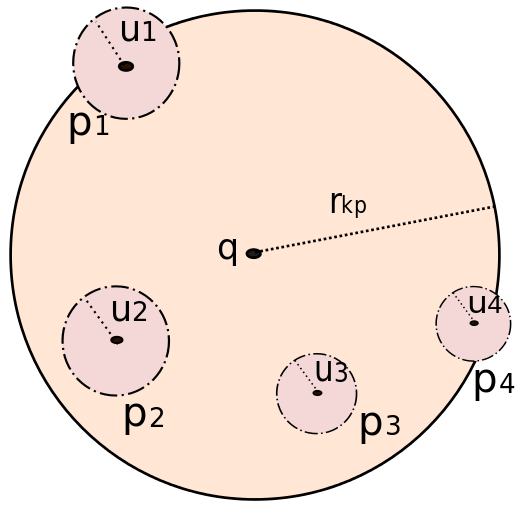
\includegraphics[width=\linewidth]{poi.png}
  \caption{Retrieved POIs within $r_{kp}$ centring $q$}\label{fig:poi}
\endminipage\hfill
\minipage{0.32\textwidth}
  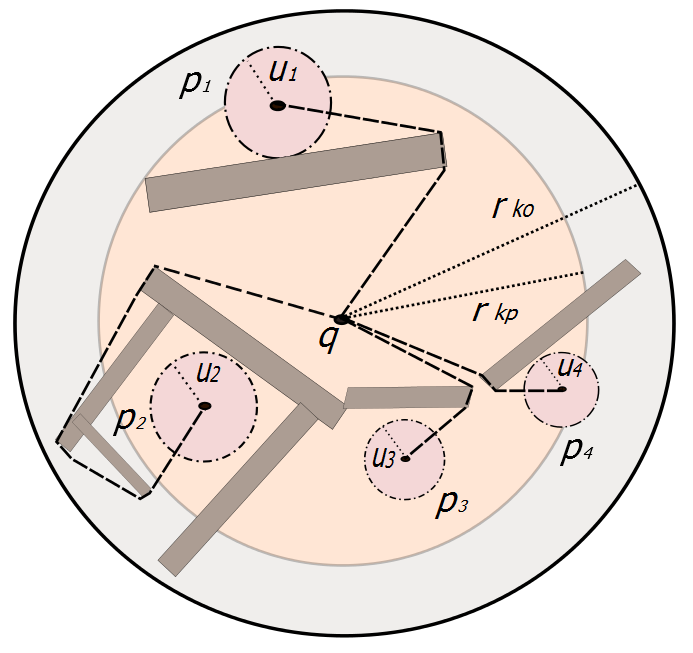
\includegraphics[width=\linewidth]{poi_obs_path.png}
  \caption{Visibility graph with all POIs and obstacles}\label{fig:poi_obs_path}
\endminipage\hfill
\minipage{0.32\textwidth}%
  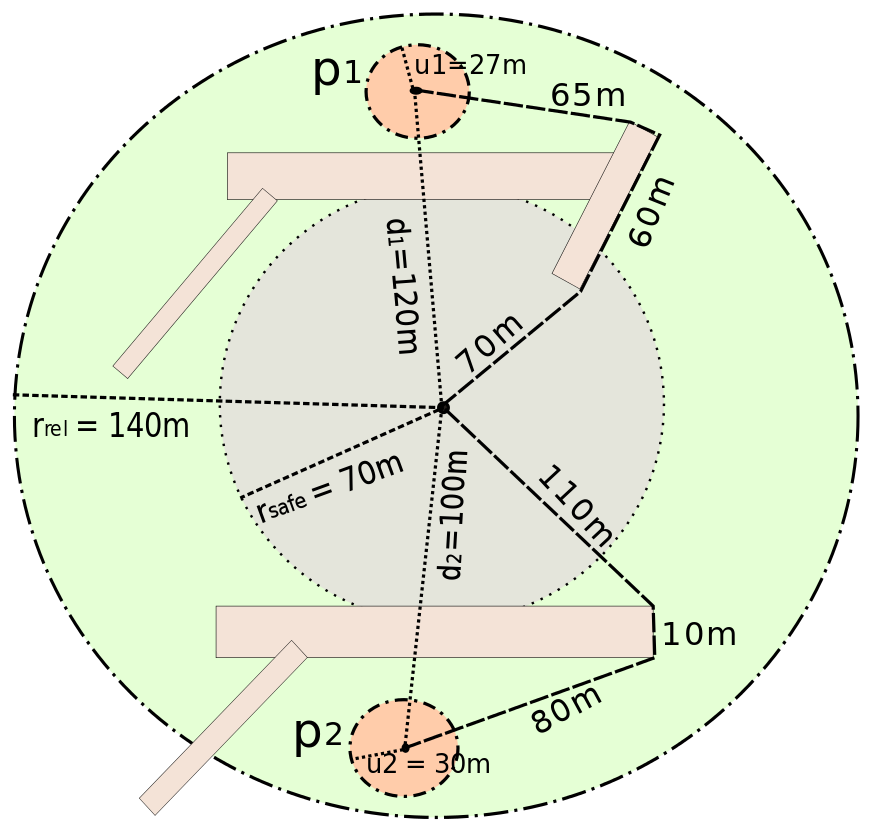
\includegraphics[width=\linewidth]{safe_region.png}
  \caption{A really Awesome Image}\label{fig:safe_region}
\endminipage
\end{figure}
%Figure \ref{fig:safe_region} Safe region Computation


The input to the algorithm \ref{ULC} is the current and the previous location of the client ($q'$ and $q$), the radius of the safe region($r_{safe}$), the reliable region($r_{rel}$) and the known region($r_{k}$) and finally the already computed answer set $A$. The output of the algorithm is the minimum distance $d_u$ to trigger this algorithm the next time.

\begin{algorithm}
\caption{UpdateOnLocChange($q, q', r_{safe}, r_{rel}, r_{kp}, r_{ko}, A$)}
\label{ULC}
%\begin{algorithmic}[5]
%\Procedure{UpdateAlarm}{}

    \SetKwInOut{Input}{Input}
    \SetKwInOut{Output}{Output}
    \Input{$q, q', r_{safe}, r_{rel}, r_{kp}, r_{ko}$}
    \Output{$d_u$}
    $q_d \gets \textsc{EuclideanDist}(q, q')$
    
    \If{$q_d > r_{rel}$}{
    		$A \gets \textsc{ClientInit}(q, q_d)$ \;
    		call \textsc{ConfigAlarm}($q, A$) \;
    }
    
    \If{$q_d > r_{safe}$}{
    		call \textsc{ConfigAlarm}($q, A$) \;
    }
    
    \Return $d_u = r_{safe}$

%\EndProcedure
%\end{algorithmic}
\end{algorithm}

\subsection{Computational Cost Saving Mode}
The algorithm runs in this mode almost similarly as the "Bandwidth Saving Mode" with all the 3 described parts - other than the algorithm \ref{ClientInit} returning the computed $V_G$ as another element of the answer set $A$ from the server side and the algorithm \ref{ConfigAlarm} not reconstructing this $V_G$ in the client side.

\subsection{Example Simulation} \label{saos_example_simu}
In figure \ref{fig:poi} an example scenario is put as if 3 POIs $p_1, p_2,$ and $p_3$ are retrieved and in the figure \ref{fig:poi_obs_path} the same case is shown as if the algorithm \ref{ClientInit} has returned the constructed visibility-graph $V_G$ along with the set of POIs $P$, obstacles $O$ and the radius of the POIs' known region $r_{kp}$ and that of the obstacles' known region $r_{ko}$.
\\ In the figure \ref{fig:safe_region}, a critical case for the algorithm \ref{ConfigAlarm} is demonstrated regarding the calculation of the safe region.
\\During the for-loop at line no. 4 of the algorithm \ref{ConfigAlarm}, the safe-region's radius is calculated to be,
\\$r_{safe} = min( (65+60+70)-27, (110+10+80)-30 ) = 168m$, whereas the safe-region is about to include both the POIs along with their whole path in the visibility graph $V_G$ from the center $q$ and also without any of them within their alarming zone. In this case as per the definition \ref{def:safe_region} , no calculation would be done to alarm the client even if s/he enters within any of the POI's alarming zone. To narrow down this false safe-region for the sake of accuracy, the condition of line no. 9 inside the foreach-loop gets true and the radius is modified as $r_{safe} = min(168, 120-27) = 93m$ for $p_1$ and in the second and final iteration for $p_2$, $r_{safe} = min( 93, 100-30) = 70m$.

\subsection{Proof of Accuracy}
The following proved facts bear the proof of accuracy and completeness of our final algorithms \ref{ClientInit}, \ref{ConfigAlarm} and \ref{ULC}.\\
In the algorithm \ref{ClientInit}, the fact that the incremental-search will find at least 1 POI and stop the increment to get a fixed $r_{kp}$ within finite time follows from the incremental search algorithm given the fact that the POI data-set is not empty.
\\One more fact is to be proved to guarantee the accuracy and completeness of the algorithm \ref{ClientInit} as - the while loop at line \ref{while} runs for a finite amount of time.

\begin{proof}
If there's no unreachable POI or no/single collision between any obstacle and the perimeter of the POIs' known region, then the loop will terminate immediately.
\\If there is any totally unreachable POI, it must be surrounded by a series of obstacles, which will certainly cause no collision (in case that all obstacles are already inside the known region) or more than one collision (in case that some parts of the series of the obstacles are inside the known region) with the perimeter of the known region. So, the second clause will be false and the loop will terminate.
\\Finally, if there is any unreachable POI which can be reached by retrieving an extended set of obstacles, then it will be done and checked inside the loop and then loop will finish its purpose within finite time.
\end{proof}

\textbf{No computation is needed to accurately give alarm while the user is inside the safe region.}\\

\begin{proof}
\textit{Case 1}: When the path to a POI is a straight line: 
In this case the claim is trivial to prove. We take $min( D_i - U_i )$ as the radius of safe region. Suppose there is a POI $P$ with alarming distance $U$. The radius of the safe region is $r$. and the users current position is $p'$. Suppose for contradiction an alarm should be triggered to the user for $P$ in his current position $p'$. Then, $|p-p'|>(D-U)$. But as the user is within the safe region, $|p-p'|<r$ . But that mean, $r>|D-U|$ which is a contradiction because the algorithm \ref{ConfigAlarm} chooses the minimum between all $(D_i - U_i )$.
\textit{Case 2:} When the path to a POI is not a straight line: 
In this case there is an obstacle in the path to the POI. There can be two cases, 
a. the safe region contains the full path to the obstructed POI 
b. The safe region does not contain the full path to the obstructed POI.
In case a, the algorithm \ref{ConfigAlarm} computes the minimum among the Euclidean distances of the POIs. As we know from the Euclidean lower bound property that the obstructed distance>= Euclidean distance. The proof follows from case 1. The safe region's radius will never over-assume the distance to the POI as it is considering the Euclidean distance.
In case b, the algorithm \ref{ConfigAlarm} chooses the safe-region radius with the assumption that as the POI's full path is not the safe region, even if the user get's close to the POI in Euclidean Distance, Obstructed distance will always be higher.(Euclidean Lower Bound)
\end{proof}

\textbf{No query to the server has to be done to correctly give any alarm while the user is inside the reliable region}\\
Recall from algorithms \ref{ClientInit} and \ref{ConfigAlarm} that the minimum alarming distance among all the available POIs for the user is returned as $U_{min}$, which is used to reduce the POIs' known region's radius to the reliable region's radius as $r_{rel}$ = $r_{ko} – U_{max}$.

\begin{proof}
If the safe region is well inside the safe region, then this proof follows the 1st fact.
The 3 procedures run simultaneously to give accurate alarm for the POIs inside the known region and so inside the reliable as well as the safe region.
The proof is needed for any POI outside both the known regions.

Let there be a POI outside both the known regions for which no alarm is triggered when the user gets inside its alarming distance Ui . 
But meanwhile, the user must cross the reliable region because $r_{ko} - r_{rel} = U_{max} > U_i$ 
So according to algorithm \ref{ULC}, algorithm \ref{ClientInit} and \ref{ConfigAlarm} are re-run and the assumed POI must come inside the newly computed known regions and its alarm will be given accurately.
Hence, there is a contradiction.
Therefore, there is no POI outside the reliable region which may miss its alarm.
So, the statement is proved.
\end{proof}

\textbf{The update procedure is run timely to re-calculate the answer set.}
\begin{proof} 
This claim follows trivially from the proof of the fact that - no computation is needed to accurately give alarm while the user is inside the safe region.
\end{proof}


\section{Conclusions}
This paragraph will end the body of this sample document.
Remember that you might still have Acknowledgments or
Appendices; brief samples of these
follow.  There is still the Bibliography to deal with; and
we will make a disclaimer about that here: with the exception
of the reference to the \LaTeX\ book, the citations in
this paper are to articles which have nothing to
do with the present subject and are used as
examples only.
%\end{document}  % This is where a 'short' article might terminate

%ACKNOWLEDGMENTS are optional
\section{Acknowledgments}
This section is optional; it is a location for you
to acknowledge grants, funding, editing assistance and
what have you.  In the present case, for example, the
authors would like to thank Gerald Murray of ACM for
his help in codifying this \textit{Author's Guide}
and the \textbf{.cls} and \textbf{.tex} files that it describes.

%
% The following two commands are all you need in the
% initial runs of your .tex file to
% produce the bibliography for the citations in your paper.
\bibliographystyle{plain}
\bibliography{lee}  % sigproc.bib is the name of the Bibliography in this case
% You must have a proper ".bib" file
%  and remember to run:
% latex bibtex latex latex
% to resolve all references
%
% ACM needs 'a single self-contained file'!
%
%APPENDICES are optional
%\balancecolumns
\appendix
%Appendix A
\section{Headings in Appendices}
The rules about hierarchical headings discussed above for
the body of the article are different in the appendices.
In the \textbf{appendix} environment, the command
\textbf{section} is used to
indicate the start of each Appendix, with alphabetic order
designation (i.e. the first is A, the second B, etc.) and
a title (if you include one).  So, if you need
hierarchical structure
\textit{within} an Appendix, start with \textbf{subsection} as the
highest level. Here is an outline of the body of this
document in Appendix-appropriate form:
\subsection{Introduction}
\subsection{The Body of the Paper}
\subsubsection{Type Changes and  Special Characters}
\subsubsection{Math Equations}
\paragraph{Inline (In-text) Equations}
\paragraph{Display Equations}
\subsubsection{Citations}
\subsubsection{Tables}
\subsubsection{Figures}
\subsubsection{Theorem-like Constructs}
\subsubsection*{A Caveat for the \TeX\ Expert}
\subsection{Conclusions}
\subsection{Acknowledgments}
\subsection{Additional Authors}
This section is inserted by \LaTeX; you do not insert it.
You just add the names and information in the
\texttt{{\char'134}additionalauthors} command at the start
of the document.
\subsection{References}
Generated by bibtex from your ~.bib file.  Run latex,
then bibtex, then latex twice (to resolve references)
to create the \cite{mur} ~.bbl file. \cite{roadalarm} Insert that ~.bbl file into
the .tex source file and comment out
the command \texttt{{\char'134}thebibliography}.
% This next section command marks the start of
% Appendix B, and does not continue the present hierarchy
\section{More Help for the Hardy}
The sig-alternate.cls file itself is chock-full of succinct
and helpful comments.  If you consider yourself a moderately
experienced to expert user of \LaTeX, you may find reading
it useful but please remember not to change it.
%\balancecolumns % GM June 2007
% That's all folks!
\end{document}
